\chapter{Facility Layer \label{chap:facilitylayer}}
\begin{figure}[htbp]
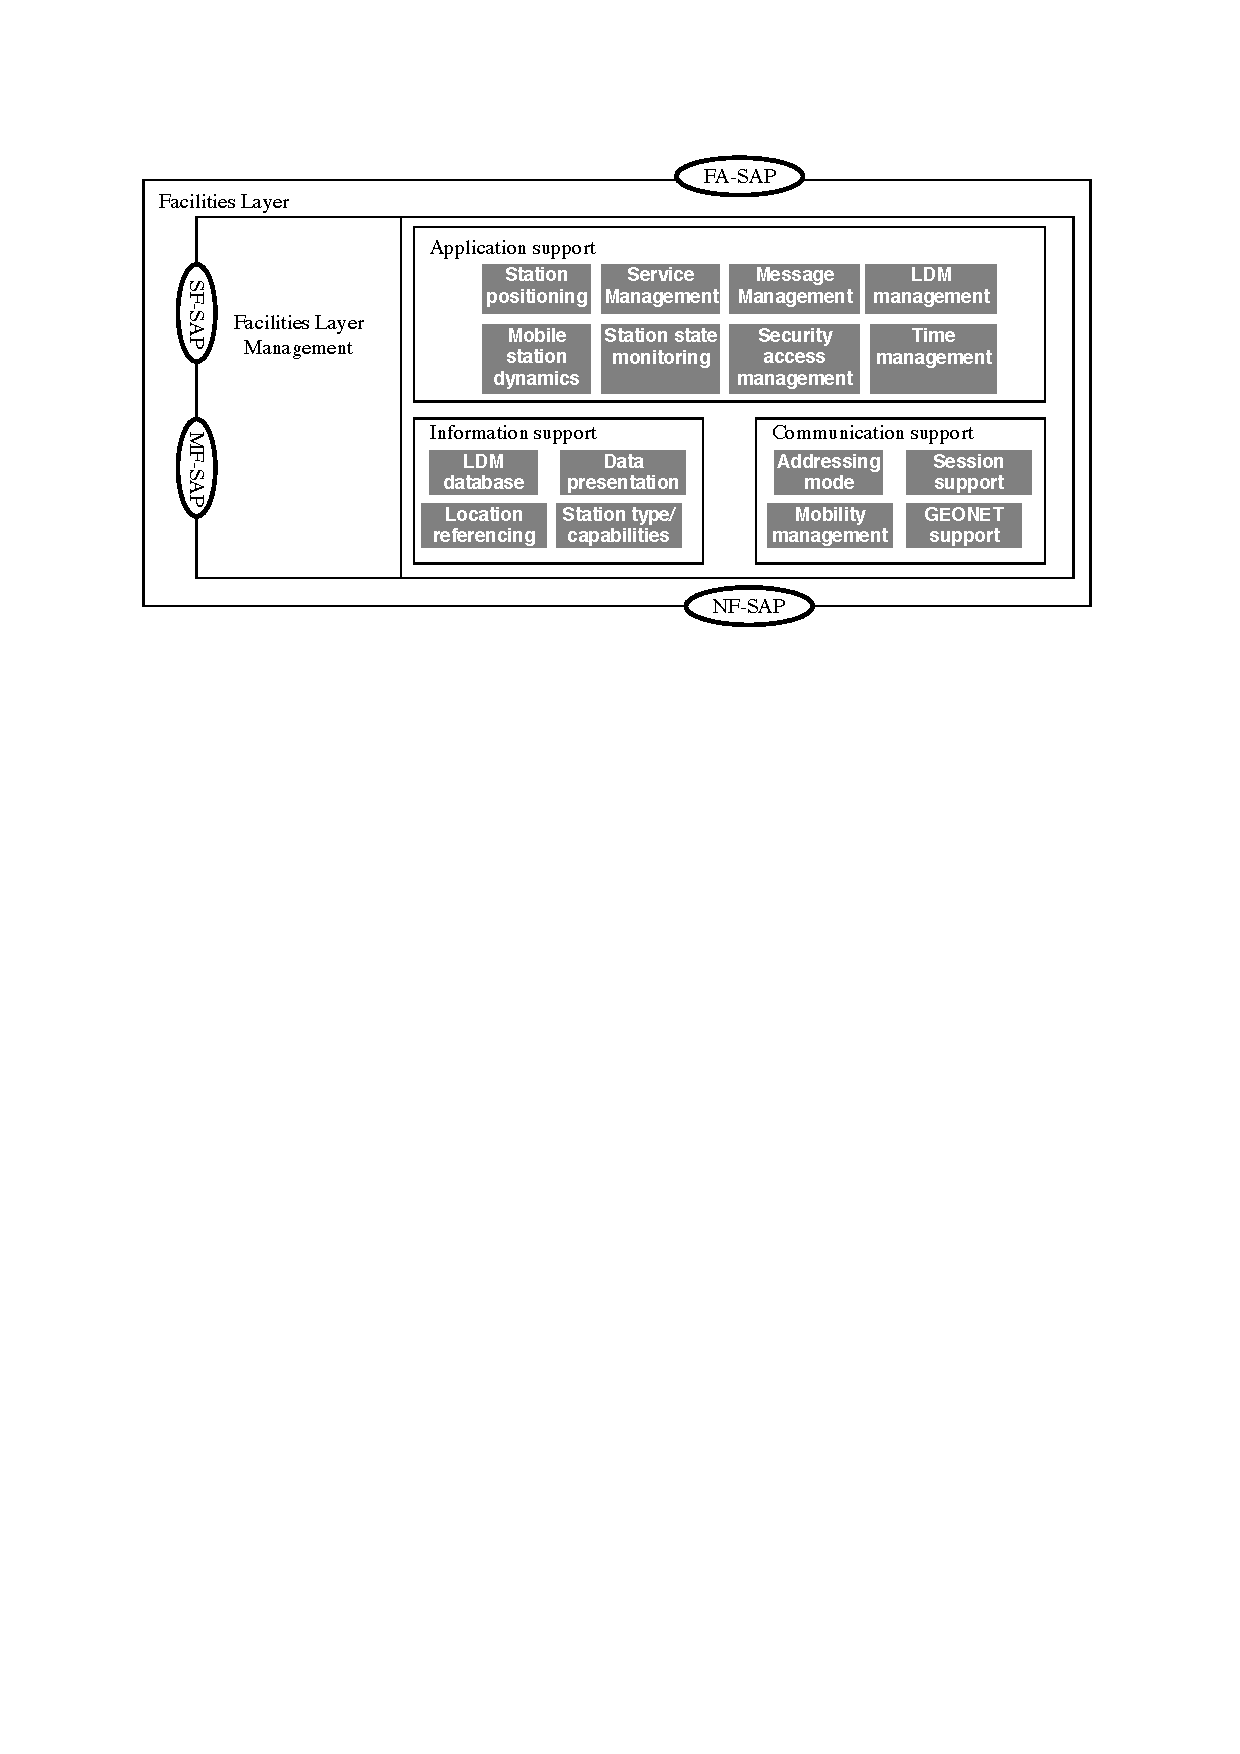
\includegraphics[width=0.99\textwidth]{content/images/04_facilitylayer/facility_layer_model.pdf}
\caption{Die Komponenten der \acl{C2C}}
\label{fig:komponentenderc2x}
\end{figure}
Der Facility Layer liegt unterhalb des Applicationlayer und teilt sich in drei Hauptkomponenten auf. Er bietet verschiedene allgemeine Services an die von den Anwendungen des Application Layer verwendet werden können.
\subsection{Application Support}

The application support is the kernel of common functions supporting the applications. This consists of
station lifecycle management, automatic services discovery, download and initialization of new services,
HMI generic capabilities, and many others. A key concept in ITS is the ability of transport entities
(vehicles, roadside infrastructure, pedestrians, etc.) to collect knowledge of their local environment, from
a range of sensor equipment, and to share that knowledge in order to make more intelligent use of the
transport infrastructure. This is described in the term "co-operative awareness". 
\subsubsection{Station positioning}
\subsubsection{Mobile station dynamic monitoring}
\subsubsection{Station state monitoring}
\subsubsection{Services management }
\subsubsection{LDM management }
\subsubsection{Messages management}
\subsubsection{Security access management}
\subsubsection{Time management}
\subsubsection{Time management}
\subsubsection{Time management}

\subsection{Information Support}
The information support covers the presentation layer of the OSI reference model and holds the role of
data management. In any ITS system, there will be an abundance of data sources, both mobile and static
ones. These data will mostly be location referenced, time specific and attached with life time value and
with accuracy and reliability parameters. Therefore, fusing data and keeping the information up to date is
one of the challenges of information support. Main entity that supports this is Local Dynamic
Map (LDM) that is able to take data both from different sources and from received ITS messages to build
a data model of the local environment. Furthermore, the information support takes on many functions of
the OSI Presentation Layer. 

\subsection{Communication Support}
The communication support, which includes the session layer of the OSI Reference model. It will
cooperate with the transport and network layer to achieve the various communication modes required by
the applications. 

\section{CAM\label{sec:cam}}

\section{DEN\label{sec:den}}


\section{SPaT\label{sec:spat}}

\section{TOPO\label{sec:topo}}
